\documentclass[border=1mm, convert]{standalone}
%\documentclass{article}
\usepackage{tikz}
\usetikzlibrary{arrows}
\usetikzlibrary{calc}

\begin{document}

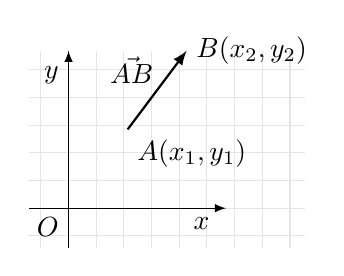
\begin{tikzpicture}[line/.style={>=latex}] 
\coordinate (A) at (.75, 1);
\coordinate (B) at (1.5, 2);

%\draw[step=10pt, color=white] (-.5, -.5) grid (2.5, 2.5);
\draw[step=10pt, color=black!10] (-.5, -.5) grid (3, 2);
\draw[->, line] (-.5, 0) -- node [below, very near end] {$x$} (2, 0);
\draw[->, line] (0, -.5) -- node [left, very near end] {$y$} (0, 2);

\node at (0,0) [below left] {$O$};
\node at (A) [below right] {$A (x_1,y_1)$};
\node at (B) [below, right] {$B (x_2,y_2)$};
\draw[->, line, thick] (A) -- node [left=3pt, near end]    {$\vec{AB}$} (B);

\end{tikzpicture}
\end{document}